% Enable warnings about problematic code
\RequirePackage[l2tabu, orthodox]{nag}

\documentclass{WeSTassignment}

% The lecture title, e.g. "Web Information Retrieval".
\lecture{Introduction to Web Science}
% The names of the lecturer and the instructor(s)
\author{%
  Prof. Dr.~Steffen~Staab\\{\normalsize\mailto{staab@uni-koblenz.de}} \and
  Ren{\'e}~Pickhardt\\{\normalsize\mailto{rpickhardt@uni-koblenz.de}} \and
   Korok~Sengupta\\{\normalsize\mailto{koroksengupta@uni-koblenz.de}}
}
% Assignment number.
\assignmentnumber{6}
% Institute of lecture.
\institute{%
  Institute of Web Science and Technologies\\%
  Department of Computer Science\\%
  University of Koblenz-Landau%
}
% Date until students should submit their solutions.
\datesubmission{December 6, 2016, 10:00 a.m.}
% Date on which the assignments will be discussed in the tutorial.
\datetutorial{December 9, 2016, 12:00 p.m.}

% Set langauge of text.
\setdefaultlanguage[
  variant = american, % Use American instead of Britsh English.
]{english}

% Specify bib file location.
\addbibresource{bibliography.bib}

% For left aligned centerd boxes
% see http://tex.stackexchange.com/a/25591/75225
\usepackage{varwidth}

% ==============================================================================
% Document

\begin{document}

\maketitle
Please look at the lessons 1) \textbf{Simple descriptive text models} \& 2) \textbf{Advanced descriptive text models}

For all the assignment questions that require you to write code, make sure to include the code in the answer sheet, along with a separate python file. Where screen shots are required, please add them in the answers directly and not as separate files.\\ \\ 

%Please mention your team Names here: 
Team Name: hotel

% ------------------------------------------------------------------------------
\section{Digging deeper into Norms (10 points)}

You have been introduced to the concept of a norm and have seen that the uniform norm $|| \cdot ||_\infty$ fullfills all three axioms of a norm which are:

\begin{enumerate}
\item Positiv definite
\item Homogeneous
\item Triangle inequality
\end{enumerate}

Recall that for a function $f:M\longrightarrow \mathbb{R}$ with $M$ being a finite set\footnote{You could for example think of the function measuring the frequency of a word depening on its rank.} we have defined the $L_1$-norm of $f$ as:

\begin{equation}
|| f ||_1 := \sum_{x\in M}|f(x)|
\end{equation}

In this exercise you should
\begin{enumerate}
\item calculate $||f - g||_1$ and $||f -g||_\infty$ for the functions $f$ and $g$ that are defined as \begin{itemize}
\item $f(0) = 2, f(1) = -4, f(2) = 8, f(3) = -4$ and 
\item $g(0) = 5, f(1) = 1, g(2) = 7, g(3) = -3$ \end{itemize}
\item proof that all three axioms for norms hold for the $L_1$-norm.
\end{enumerate}


\subsection{Hints:}
\begin{enumerate}
\item The proofs work in a very similar fashion to those from the uniform norm that was depicted in the videos. 

\item You can expect that the proofs for each property also will be "three-liners".

\item Both parts of this exercise are meant to practice proper and clean mathematical notation as this is very helpfull when reading and understanding research papers. Discuss in your study group not only the logics of the calculation and the proof (before submission) but try to emphasize on the question whether your submission is able to communicate exactly what you are doing. 

\end{enumerate}
\newpage
\textbf{Answer:}

$f: M \rightarrow \mathbb{R}$\\
\noindent
\begin{align*}
||f||_1 := \sum_{x \in M}{|f(x)|}
\end{align*}\\
\[||f||_\infty := \sup_{x \in M} ||f(x)||_\mathbb{R} = \sup \{|f(x)| : x \in M\}\]\\
\\
f(0) = 2, f(1) = -4, f(2) = 8, f(3) = -4\\
g(0) = 5, g(1) = 1, g(2) = 7, g(3) = -3\\
\\
\[||f-g||_1 = \sum_{x \in M}{|f(x) - g(x)|}\]\\
= $| 2-5| + |-4 -1| + |8-7| + |-4 - (-3)|$\\
= $ 3 + 5 + 1 + 1$\\
= 10\\
\\
\[||f-g||_\infty = \sup_{x \in M} ||f(x) - g(x)||_\mathbb{R} = \sup \{|f(x) - g(x)| : x\in M\}\]\\
\\
$|f(0) - g(0)| = |2 - 5| = 3$\\
$|f(1) - g(1)| = |-4 - 1| = 5$\\
$|f(2) - g(2)| = |8 - 7| = 1$ \\
$|f(3) - g(3)| = |-4 - (-3)| = 1$\\
\[\rightarrow \sup_{x \in M} ||f(x) - g(x)||_\mathbb{R} = 5\]\\
\\
\subsubsection*{Positive definite}
Assumption: $||f||_1 = 0 \Rightarrow f = 0$\\
\\
Proof:\\
\[||f||_1 =  0 \Leftrightarrow \sum_{x \in M}{|f(x)|} = 0\] \\
\[ \Rightarrow \sum_{x \in M} {|f(x)|} = 0\] \\
$ \Rightarrow| f(0)| + |f(1)| + ... + |f(x)| = 0$ \\
$ \Rightarrow f(x) = 0~\forall x$ \\
$\Rightarrow f = 0$

\subsubsection*{Homogeneous}
Assumption: $||\alpha f||_1 = |\alpha|~||f||_1, \alpha \in \mathbb{R}$\\
\\
Proof:\\
\[||\alpha f||_1 := \sum_{x \in M}{|\alpha|~|f(x)|}\]\\
\[\Rightarrow \sum_{x \in M}{|\alpha|~|f(x)|} = |\alpha| \cdot |f(0)| + |\alpha| \cdot |f(1)| + ... + |\alpha| \cdot |f(x)\] \\
$\Rightarrow |\alpha| \cdot ( |f(0)| + |f(1)| + ... + |f(x)|)$ \\
\[\Rightarrow |\alpha| \cdot \sum_{x \in M}{ |f(x)|}\] \\
$\Rightarrow |\alpha|~||f||_1$\\
Since $\alpha$ has to be positive for our usage, we can write $\alpha$ instead of $|\alpha|$ and thus gain: $\alpha ||f||_1$
\newpage
\subsubsection*{Triangle inequality}
Assumption: $||f + g||_1 \leq ||f||_1 + ||g||_1$\\
\\
Proof: \\
\[ \sum_{x \in M}{|f(x) + g(x)|} \leq (\sum_{x \in M} {|f(x)|})  + |g(x)| \leq \sum_{x \in M} {|f(x)|} +  \sum_{x \in M} {|g(x)|} = ||f||_1 + ||g||_1\]



% ------------------------------------------------------------------------------
\section{Coming up with a research hypothesis (12 points)}
You can find all the text of the articles from Simple English Wikipedia at \url{http://141.26.208.82/simple-20160801-1-article-per-line.zip} each line contains one single article. 

In this task we want you to be creative and do some research on this data set. The ultimate goal for this exercise is to practice the way of coming up with a research hypothesis and testable predictions. 

In order to do this please \textbf{shortly}\footnote{Depending on the question shortly could mean one or two sentences or up to a thousand characters. We don't want to give a harsh limit because we trust in you to be reasonable.} answer the following questions: 

\begin{enumerate}
\item What are some obervations about the data set that you can make? State at least three obervations.
\item Which of these observations make you curious and awaken your interest? Ask a question about why this pattern could occur.
\item Formulate up to three potentiel research hypothesis.
\item Take the most promesing hypothesis and develop testable predictions.
\item Explain how you would like to use the data set to test the prediction by means of descriptive statistics. Also explain how you would expect your outcome. 

(If you realize that the last two steps would not lead anywhere repeat with one of your other research hypothesis.)
\end{enumerate}

\subsection{Hints:}
\begin{itemize}
\item The first question could already include some diagrams (from the lecture or ones that you did yourselves).
\item In step 3 explain how each of your hypothesis is falsifiable. 
\item In the fifth step you could state something like: "We expect to see two diagrams. The first one has ... on the x-axis and ... on the y-axis. The image should look like a ... The second diagram ...". You could even draw a sketch of the diagram and explain how this would support or reject your testable hypothesis. 
\end{itemize}

\textbf{Answer:}
\\
1. 
\begin{itemize}
	\item Not every article contains quotation marks 
	\item Not every article contains parenthesis 
	\item More than one article contains numbers
	\item Articles contain vowels and consonants
	\item The length of the articles differ 
	\item Many articles start with an article
\end{itemize}
2.
The most interesting would be the start of an article, as there the user decides wether to continue reading or not.
\\3. 
\begin{itemize}
	\item In the whole article text of the Simple English Wikipedia are more occurrences of vowels than consonants. \\ This hypothesis is false if there are more consonants than vowels in the article texts of the Simple English Wikipedia.
	\item In the whole article text of the Simple English Wikipedia are more occurrences of letters than numbers. \\ This hypothesis is false if there are more occurrences of numbers than letters in the article texts of the Simple English Wikipedia.
	\item In the Simple English Wikipedia more than 30\% of article texts start with a definite or indefinite article. \\ This hypothesis is false if 50\% or less of the opening words in the article texts of the Simple English Wikipedia are articles. 
\end{itemize}
4. 
We choose hypothesis three: "In the Simple English Wikipedia more than 30\% of article texts start with a definite or indefinite article.". The hypothesis is already testable.\\
5.
We will extract every opening word of each article. Then we will compare it to a list of articles\footnote{a, an, the} not regarding upper and lower case. If the opening word matches, we will increase a counter. Finally, we will divide the counter by the total number of articles. Therefore we have the percentage of articles starting with an article. 
We expect our outcome to have a deviation of +/- 5\%.

% ------------------------------------------------------------------------------


\section{Statistical Validity (8 points)}
In the above question, you were asked to formulate your hypothesis. In this one, you should follow your own defined roadmap from task 2 validate (or reject) your hypothesis. 

\subsection{Hints:}
\begin{itemize}
\item In case feel uncomfortable to test one of the predictions from task 2 you can "steal" one of the many hypothesis (and with them imlicitly associated testable predictions) or diagrams depicted from the lecture and reproduce it. However in that case you cannot expect to get the total amount of points for task 3. 
\end{itemize}

\textbf{Answer:}
\\
Out of 119,753 articles 24,304 started with a definite or indefinite article. This corresponds to a percentage of 20.3\%.

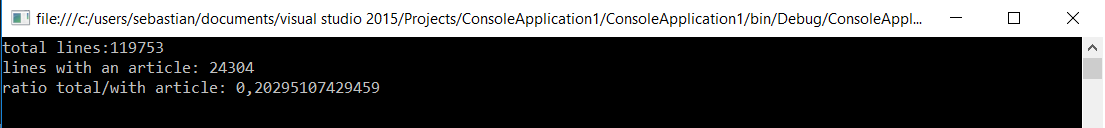
\includegraphics[width=450px]{articleRatio}

% ------------------------------------------------------------------------------






\makefooter

\end{document}
